\chapter{Dvodimenzionalne vložitve podatkov}

V tem poglavju obravnavamo metode, ki primere vložijo v dvodimenzionalni prostor, tako da geometrijski odnosi med točkami čim bolje odražajo odnose med primeri v izvirnem prostoru. Takšne vložitve uporabljamo predvsem za prikaz strukture podatkov v namene odkrivanja zanimivih vzorcev in skupin, pa tudi v namene rangiranja in odkrivanja odnosov med posameznimi primeri iz učne množice.

Analiza glavnih komponent, o kateri smo govorili v prejšnjem poglavju, ni vložitev v istem smislu kot metode, obravnavane v tem poglavju. Metoda glavnih komponent je projekcijska metoda, ki oblikuje matematični predpis, recimo \( U \) (matrika, sestavljena iz smernih vektorjev glavnih komponent \( u_1 \) in \( u_2 \)), ki podatke \( X \) projicira v dve dimenziji, torej \( Z = XU \). Projekcija v splošnem ni isto kot vložitev. Pri PCA iščemo preslikavo \( f(x) \), ki podatke projicira v nov koordinatni sistem, pri metodah, obravnavanih v tem poglavju, pa iščemo neposredno postavitev točk \( y_1, \dots, y_n \in \mathbb{R}^2 \),
%
\marginnote{Oznaka $y_i$ tu ne predstavlja razreda (kot pri napovednih modelih), temveč koordinate točke v vložitvi primera $x_i$ oziroma položaj tega primera v dvodimenzionalnem prostoru.}
%
ki čim bolje ohranja izbrane odnose med primeri. Zato takšne metode praviloma ne podajo enostavne preslikave za nove podatke v isti prostor.

Ogledali si bomo tri pristope k dvodimenzionalnim vložitvam podatkov: večrazsežno lestvičenje (MDS), metodo t-SNE in vložitve s silami. Prva je pomembna z zgodovinskega vidika, druga poudarja lokalno strukturo podatkov, tretja pa izhaja iz vizualizacije omrežij. Pri majhnih podatkovnih množicah so lahko vložitve MDS, t-SNE in metod s silami podobne, pri večjih in visokorazsežnih podatkih pa pridejo razlike med pristopi precej bolj do izraza.

Skupen vsem trem opisanim metodam je osnovni pristop vložitve primerov v dve dimenziji. Uporabili bomo kriterijsko funkcijo, ki izhaja iz razdalj med primeri v izvornem prostoru in jih na ustrezen način poveže s položaji točk v vložitvenem prostoru. Začetno vložitev dobimo tako, da točke (primere) v ravnini razporedimo naključno, nato pa njihove položaje postopoma popravljamo v smeri gradienta kriterijske funkcije glede na koordinate teh točk. Tokrat torej model ne predstavljajo uteži ali parametri preslikave, temveč kar same koordinate točk v vložitvi, zato je število parametrov enako $2n$, kjer je $n$ število primerov.

\section{Podatki}


Začnimo kar s podatki.
%
\marginnote{Podatke lahko v tem poglavju opišemo zgolj z razdaljami med primeri, brez eksplicitnega atributnega zapisa. Tak opis pa ni neposreden vhod za PCA, saj ta metoda potrebuje predstavitev primerov z atributi.}
%

Vse metode, ki jih bomo v tem poglavju predstavili, lahko izhajajo iz razdalj ali podobnosti med primeri. Predpostavili bomo, da so ti odnosi že podani. Tokrat primerov torej ne bomo opisovali eksplicitno z atributi, kot smo bili vajeni v prejšnjih poglavjih, temveč zgolj z razdaljami med njimi. Te razdalje bi običajno zapisali v (simetrični) matriki, lahko pa jih predstavimo tudi s spodnjim slovarjem:

\vspace*{3mm}
\begin{lstlisting}
distances = {
    ("Novo Mesto", "Maribor"): 170,
    ("Novo Mesto", "Celje"): 83,
    ("Novo Mesto", "Koper"): 169,
    ("Novo Mesto", "Kranj"): 99,
    ("Novo Mesto", "Ljubljana"): 72,
    ("Novo Mesto", "Postojna"): 116,

    ("Maribor", "Celje"): 55,
    ("Maribor", "Koper"): 232,
    ("Maribor", "Kranj"): 156,
    ("Maribor", "Ljubljana"): 128,
    ("Maribor", "Postojna"): 178,

    ("Celje", "Koper"): 183,
    ("Celje", "Kranj"): 105,
    ("Celje", "Ljubljana"): 77,
    ("Celje", "Postojna"): 130,

    ("Koper", "Kranj"): 128,
    ("Koper", "Ljubljana"): 107,
    ("Koper", "Postojna"): 58,

    ("Kranj", "Ljubljana"): 30,
    ("Kranj", "Postojna"): 77,

    ("Ljubljana", "Postojna"): 53,
}
\end{lstlisting}

\section{Večrazsežno lestvičenje}

Zapišimo 
%
\marginnote{Večrazsežno lestvičenje (angl.~\emph{multidimensional scaling}, MDS) so razvili Torgerson (1952), Shepard (1962) in Kruskal (1964) v okviru psihometrije, področja, ki se ukvarja z merjenjem psiholoških lastnosti (npr. zaznav, podobnosti med dražljaji in preferenc) z uporabo statističnih metod.}
%
razdaljo med primeroma \( i \) in \( j \) z \( d_{ij} \). V večrazsežnem lestvičenju želimo primere urediti v dvodimenzionalnem prostoru tako, da vsak primer \( i \) opišemo s koordinatama \( y_i = (y_{i1}, y_{i2}) \in \mathbb{R}^2 \). V tem ciljnem prostoru naj bo razdalja med primeroma evklidska,
\[
\|y_i - y_j\| = \sqrt{(y_{i1} - y_{j1})^2 + (y_{i2} - y_{j2})^2},
\]
torej takšna, kot bi jo dobili pri običajnem razsevnem diagramu.

Cilj večrazsežnega lestvičenja 
%
\marginnote{Izraz \emph{lestvičenje} (angl. \emph{scaling}) pomeni razporejanje objektov na lestvico tako, da razdalje med njimi odražajo njihove medsebojne razlike ali podobnosti. Pridevnik \emph{večrazsežno} (angl.~\emph{multidimensional}) poudarja, da te lestvice ne tvorimo le v eni dimenziji, temveč v večrazsežnem prostoru, najpogosteje v dveh ali treh dimenzijah.}
%
je čim bolje ohraniti dane razdalje, torej naj bodo razdalje \( \|y_i - y_j\| \) v vložitvenem prostoru čim bližje izhodiščnim razdaljam \( d_{ij} \). Skladno s tem večrazsežno lestvičenje minimizira kriterijsko funkcijo
\[
J(Y) = \sum_{i < j} \bigl( \|y_i - y_j\| - d_{ij} \bigr)^2,
\]
kjer \( Y = \{y_1, \dots, y_n\} \) predstavlja iskano postavitev točk v ravnini.

Evklidska razdalja v vložitvenem prostoru je torej v celoti odvisna od položajev točk, ki predstavljajo primere; ti položaji pa so tudi parametri našega modela. Te bomo iskali z gradientnim sestopom, pri čemer bomo uporabili strojno odvajanje. Knjižnico za strojno odvajanje in učenje z gradientnim sestopom smo že zgradili v prejšnjih poglavjih, zato tu podajamo le kodo razreda za predstavitev modela večrazsežnega lestvičenja.

\vspace*{3mm}
\begin{lstlisting}
class MDS:
    def __init__(self, items):
        random.seed(100)
        self.pos = {i: [Value(random.uniform(-1, 1)) for _ in range(2)]
                    for i in sorted(items)}
    
    def parameters(self):
        return [p for pos in self.pos.values() for p in pos]
    
    def d(self, a, b):
        return sum([(ai - bi) ** 2 for ai, bi in \
                    zip(self.pos[a], self.pos[b])]) ** 0.5

    def loss(self, xs, ys):
        n = len(xs)
        return sum((self.d(*pair) - y) ** 2 \
                   for pair, y in zip(xs, ys)) / Value(n)
\end{lstlisting}

Razred \texttt{MDS} zgradi računski graf kriterijske funkcije za večrazsežno lestvičenje za dane vhodne podatke (razdalje). Vsakemu primeru priredimo naključno začetno pozicijo v ravnini (\texttt{self.pos}), te koordinate pa predstavljajo parametre modela. Metoda \texttt{d} izračuna evklidsko razdaljo med dvema primeroma v trenutni vložitvi, \texttt{loss} pa meri odstopanje med temi razdaljami in podanimi razdaljami \( d_{ij} \). 

Z gradientnim sestopom nato popravljamo položaje točk tako, da se ta napaka čim bolj zmanjša:

\vspace*{3mm}
\begin{lstlisting}
items = sorted(list(set(i for pair in distances.keys() for i in pair)))
pairs = list(distances.keys())
targets = [distances[p] for p in pairs]

model = MDS(items)
model = train(model, pairs, targets, n_epochs=1000, 
              learning_rate=0.1, report_every=100)
\end{lstlisting}

Mest je v naši učni množici malo, optimizacija pa konvergira hitro. Namesto izpisa pozicij posameznih mest je tu seveda bolj na mestu izris podatkovne karte:

\vspace*{3mm}
\begin{lstlisting}
plt.figure(figsize=(4, 4))
for city in sorted(items):
    x, y = model(city)
    plt.scatter(x.data, y.data, color="k", s=10)
    plt.annotate(
        city,
        (x.data, y.data),
        xytext=(0, 4),
        textcoords="offset points",
        ha="center",
        va="bottom",
    )
plt.savefig("mds-cities.pdf")
\end{lstlisting}

Karto mest prikazuje slika~\ref{fig:mds}.
%
\marginnote{Našo karto slovenskih mest bi lahko za lažjo primerjavo s geografskimi kartami, na katere smo navajeni, zasukali za 180 stopinj.}
%
Malce je zasukana in narobe obrnjena, a kdo pravi, da mora biti sever na vrhu in da gledamo od zgoraj. Relacije med mesti so sicer kar prave. Maribor, Celje, Ljubljana, Postojna in Koper so na glavni diagonali v pravem vrstnem redu, Kranj malce stran, Novo mesto na drugi strani. Vhodni podatki so vsebovali cestne razdalje med mesti, ki niso enake zračnim; evklidska razdalja v prostoru vložitve pa ustreza zračni. Najbrž je to glavni izvor za kakšne manjše napake, a v splošnem nam je rekonstrukcija pozicije slovenskih mest iz cestnih razdalj dobro uspela.

\begin{marginfigure}
    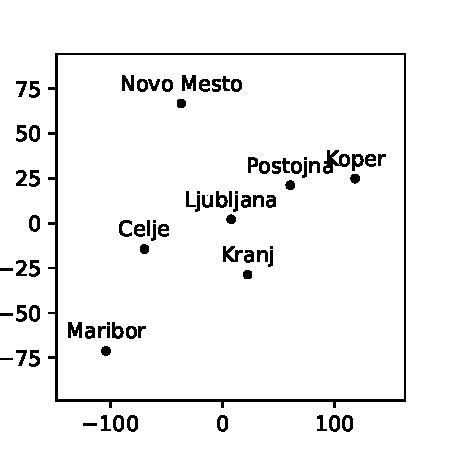
\includegraphics[width=\linewidth]{figs/060-mds-cities.pdf}
    \caption{Dvodimenzionalna vložitev z večrazsežnim lestvičenjem.}
    \label{fig:mds}
\end{marginfigure}

Opozorilo sicer: MDS-vložitev z enako dobro vrednostjo kriterijske funkcije $J(Y)$ je nešteto. Pri nespremenjeni vrednosti kriterijske funkcije vložitve lahko poljubno rotiramo in zrcalimo. Vse te transformacije ohranjajo razdalje in pravzaprav samo te nastopajo v kriterijski funkciji. Dobljene osi zato nimajo pomena in jih kot takih ne moremo povezati s kakšno razlago. Drugače kot pri PCA torej. A spomnimo: pri PCA izhajamo iz atributno predstavljenih primerov, tu pa, pri MDS, iz razdalj.

\begin{exercise}{Ista struktura, drugačen zemljevid.}
Isto podatkovno množico večkrat vloži z različnimi naključnimi začetnimi položaji ter primerjaj končne vložitve, njihove vrednosti izgube in medsebojne razdalje, da ugotoviš, koliko je rezultat odvisen od inicializacije.
\end{exercise}

\begin{exercise}{Koliko razdalj potrebujemo za zemljevid?}
Vzemi podatke o slovenskih mestih iz poglavja. Najprej uporabi vse podane razdalje in z MDS rekonstruiraj zemljevid. Nato naključno odstranjuj vedno več razdalj (npr.\ 10\%, 25\%, 50\%, 75\%) in opazuj, kako se spreminja kakovost vložitve. Kdaj postane problem premalo določen? Ali obstajajo razdalje, katerih odstranitev bistveno bolj škodi kot odstranitev drugih? Kakovost vložitve lahko opazuješ izkustveno, s karto, lahko pa uporabiš tudi isto metriko kot pri ocenjevanju izgube pri MDS, le da to oceno izračunaš iz celotne množice podatkov (torej ne samo iz te, iz katerih iz vzorčil učno množico).
\end{exercise}

\begin{exercise}{Odpornost vložitev na šum.}
    Na podatkih o cestnimi razdaljami slovenskih mest izberi eno od razdalj ter njej umetno dodaj veliko napako (npr.\ razdaljo Ljubljana--Koper povečaj za 100~km). Nato ponovno izračunaj MDS-vložitev in primerjaj položaje mest pred in po spremembi. Poskus ponovi za več velikosti napake in kasneje na več različnih parov mest. Kako se na napake odziva večrazredno lestvičenje? Katere napačne meritve najbolj pokvarijo vložitev?
\end{exercise}
    

\section{Vložitve sosedov}

Večrazsežno lestvičenje ima skriti problem: kriterijska funkcija kvadrira razliko razdalj iz vhodnih podatkov in vložitvenega prostora. Učenje modela z gradientnim sestopom se bo zato bolj ``potrudilo'' pri zmanjševanju večjih odstopanj. Če odstopanja merimo v deležih, na primer v odstotkih, in če na primer na vložitvi razdalje odstopajo od vhodnih za $10\%$, bo odstopanje med Ljubljano in Kranjem imelo dosti manjši vpliv na učenje kot odstopanje med Koprom in Mariborom. MDS torej teži k ohranjanju predvsem tistih večjih razdalj. Vpliv krajših razdalj med sosednjimi primeri je veliko manjši.

Ohranjanje večjih razdalj je seveda zaželeno, če želimo pridobiti podatkovne karte s primernimi globalnimi ureditvami. A mnogokrat nas pri podatkovni analitiki zanimajo predvsem soseščine in na podatkovnih kartah morda iščemo samo skupine podatkov ter jih skušamo interpretirati, pri čemer nas globalni odnosi oziroma skupine, ki so oddaljene druga od druge, ne zanimajo. Tako bi nas zanimale vizualizacije, kjer so izražene skupine primerov, ki so si med sabo podobni, in nas sama interpretacija razdalje med skupinami, ki so si med seboj oddaljene, ne zanima. Taka vizualizacija je na primer prikazana na sliki~\ref{fig:mds-tsne} na desni strani in je očitno zelo različna od vizualizacije istih podatkov, kot jo pridela MDS.

\begin{figure}
    \centering
    \fbox{%
        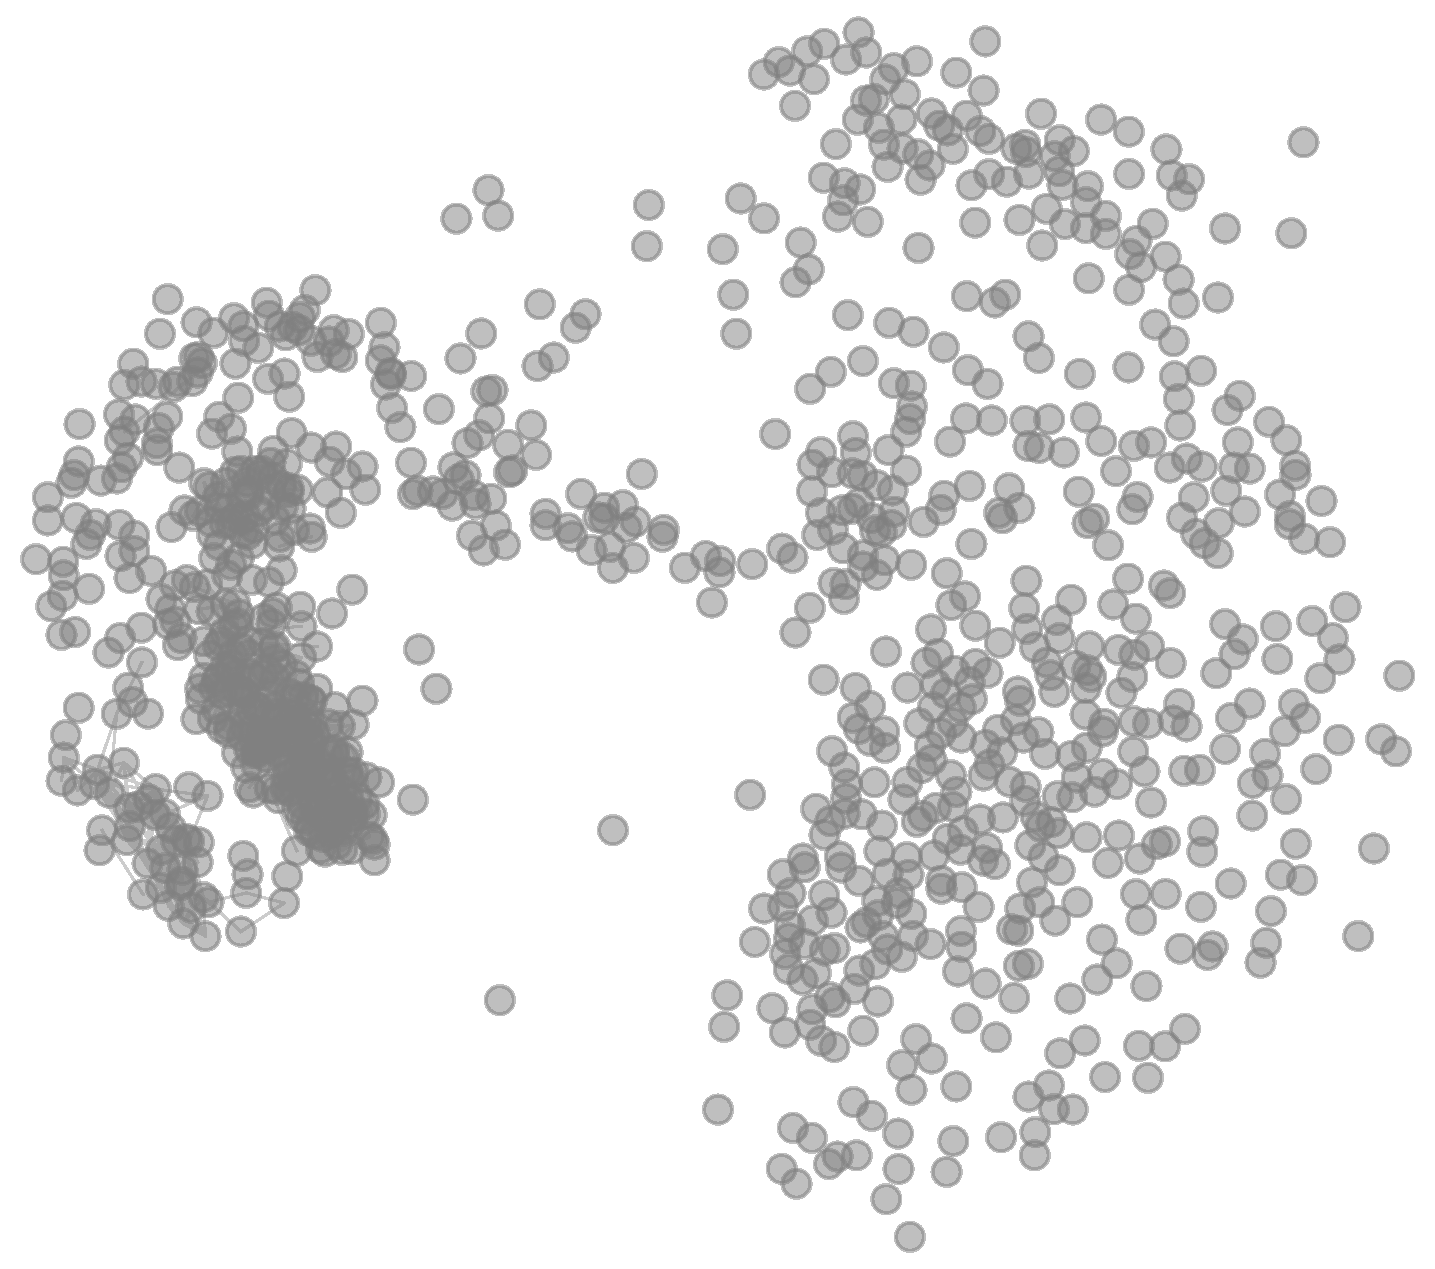
\includegraphics[width=0.45\textwidth]{figs/060-mds-bone-marrow.pdf}
    }
    \hfill
    \fbox{%
        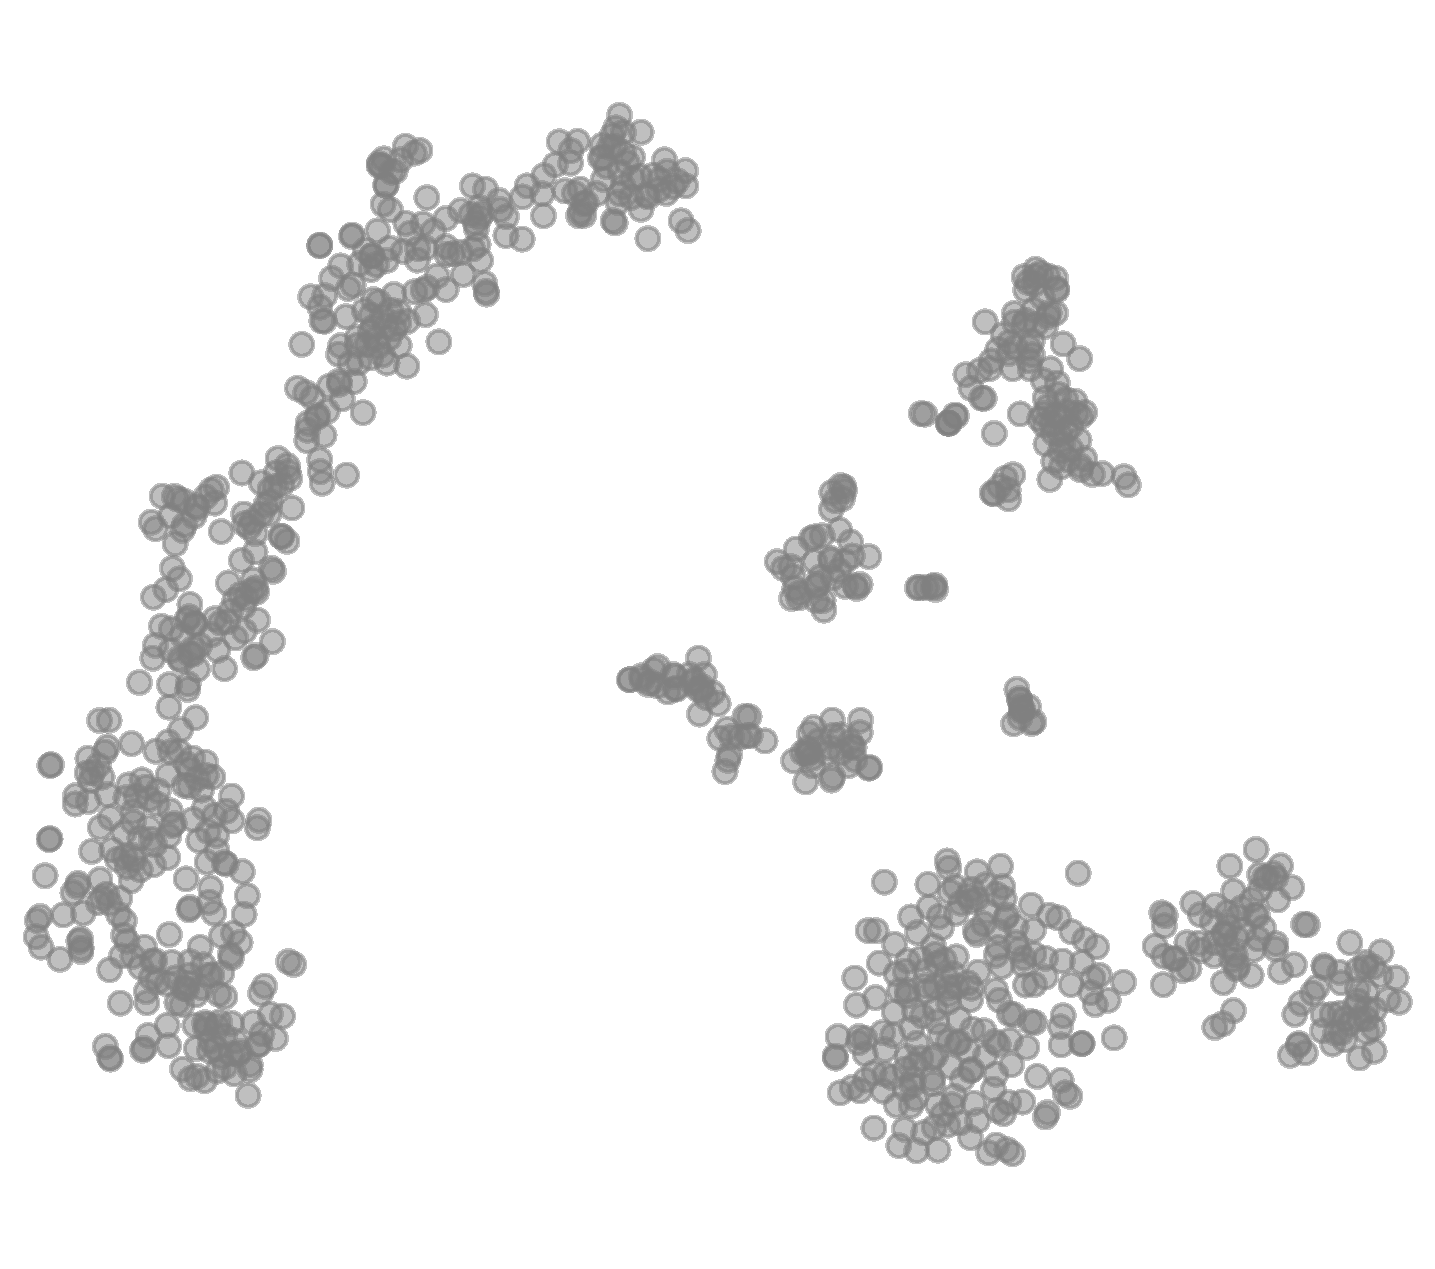
\includegraphics[width=0.45\textwidth]{figs/060-t-sne-bone-marrow.pdf}
    }
    \caption{Primerjava vložitev MDS (levo) in t-SNE (desno) na podatkih o izražanju genov v celicah kostnega mozga (vzorec tisoč celic in izrazi tisoč genov). Skupine točk naj bi pripadale posameznim celičnim tipom.}
    \label{fig:mds-tsne}
\end{figure}

Zanima nas torej ohranjanje soseščine. Za to potrebujemo mero, ki pove, kako blizu so si primeri v izvornem prostoru, in mero, ki pove, kako blizu so si v prostoru vložitev. Ti meri morata zanemariti primere, ki so si daleč, in se osredotočiti le na bližnje primere. Tu lahko uporabimo trik: namesto razdalje bomo ocenili verjetnost, da sta si dva primera blizu, v izvornem prostoru in prostoru vložitev, kot kriterijsko funkcijo pa ocenili podobnost med tema vektorjema verjetnosti, kjer z vektorjema mislimo seznama verjetnosti bližine vseh parov primerov.

Lotimo se tega bolj formalno. Kot pri MDS naj bo $x_i$ primer v izvornem prostoru in $y_i$ njegova predstavitev v vložitvi. Za vsak par primerov $(i,j)$ določimo podobnost v izvornem prostoru kot pogojno verjetnost
\[
p_{j|i} = \frac{\exp\!\left(-\frac{\|x_i - x_j\|^2}{2\sigma_i^2}\right)}{\sum_{k \ne i} \exp\!\left(-\frac{\|x_i - x_k\|^2}{2\sigma_i^2}\right)}.
\]
Ta verjetnost pove, kako verjetno bi izbrali primer $j$ kot soseda primera $i$. Pri tem parameter $\sigma_i$ določa ``širino'' okolice okoli $x_i$. Ker pogojne verjetnosti \( p_{j \mid i} \) na splošno niso simetrične, torej praviloma ne velja \( p_{j \mid i} = p_{i \mid j} \), ju pri t-SNE združimo v simetrično skupno verjetnost
\[
p_{ij} = \frac{p_{j \mid i} + p_{i \mid j}}{2n},
\]
kjer je \( n \) število vseh primerov.

V prostoru vložitev podobno določimo verjetnosti bližine, vendar uporabimo porazdelitev z debelejšimi repi (Studentovo $t$-porazdelitev z eno stopnjo prostosti):
\[
q_{ij} = \frac{\left(1 + \|y_i - y_j\|^2\right)^{-1}}{\sum_{k \ne l} \left(1 + \|y_k - y_l\|^2\right)^{-1}}.
\]
Ta izbira zmanjša problem zgoščanja, saj omogoča izrazitejšo predstavitev večjih razdalj v vložitvi kot pri Gaussovi porazdelitvi.

Cilj tega pristopa je poiskati takšne vložitve $y_i$, da so porazdelitve $p_{ij}$ in $q_{ij}$ čim bolj podobne. To dosežemo z minimizacijo Kullback-Leiblerjeve divergence:
\[
\mathcal{L}(Y) = \sum_{i \ne j} p_{ij} \log \frac{p_{ij}}{q_{ij}}.
\]
Ta kriterijska funkcija kaznuje predvsem primere, kjer sta si točki v izvornem prostoru blizu (velik $p_{ij}$), v vložitvi pa daleč narazen (majhen $q_{ij}$), zato spodbuja ohranjanje lokalne strukture podatkov.

Kriterijsko funkcijo,
%
\marginnote{Metodo SNE sta predlagala Geoffrey E. Hinton in Sam T. Roweis (2002), t-SNE pa Hinton in Laurens van der Maaten (2008). Hinton je tudi eden od očetov sodobne umetne inteligence in je leta 2024 za svoje raziskovalno delo prejel Nobelovo nagrado.}
%
kot je določena zgoraj, uporablja metoda t-SNE (angl.~\emph{t-distributed Stochastic Neighbor Embedding}). Ta pristop je nadgradil starejšo metodo SNE, ki je prav tako temeljila na primerjavi verjetnostnih porazdelitev bližin med pari primerov v izvornem prostoru in prostoru vložitev. A je imel SNE nekaj pomembnih pomanjkljivosti. Prvič, uporabljal je nesimetrične verjetnosti $p_{j|i}$ in $q_{j|i}$, kar je otežilo optimizacijo in interpretacijo. Drugič, zaradi uporabe Gaussove porazdelitve tudi v prostoru vložitev je trpel za t.~i.\ problemom ``zgoščanja'' (angl.~\emph{crowding problem}), kjer se večje razdalje težko ustrezno predstavijo v nizkodimenzionalnem prostoru, zato se točke pogosto preveč nagnetejo skupaj.

Metoda t-SNE odpravi glavni pomanjkljivosti metode SNE na dva načina: uporabi simetrično podobnost \( p_{ij} \) in v prostoru vložitve uvede Studentovo \( t \)-porazdelitev.

V nadaljevanju ne bomo implementirali celotne standardne različice metode t-SNE, temveč poenostavljeno različico, ki ohrani osnovno idejo: bližnji pari v izvornem prostoru naj imajo visoko verjetnost tudi v prostoru vložitve, kriterijska funkcija pa naj meri razliko med obema porazdelitvama. 

\vspace*{3mm}
\begin{lstlisting}
class tSNE:
    def __init__(self, items, sigma=40.0, eps=1e-12):
        random.seed(100)
        self.pos = {
            i: [Value(random.uniform(-1, 1)) for _ in range(2)]
            for i in sorted(items)
        }
        self.sigma = sigma  # constant bandwidth of the Gaussian
        self.eps = eps  # parameter for numerical stability

    def parameters(self):
        return [p for pos in self.pos.values() for p in pos]

    def p_distribution(self, pairs, distances):
        unnorm = []
        for d in distances:
            pij = math.exp(-(d ** 2) / (2 * self.sigma ** 2))
            unnorm.append(pij)

        z = sum(unnorm) + self.eps
        return [p / z for p in unnorm]

    def sqdist(self, a, b):
        return sum((ai - bi) ** 2 \
                   for ai, bi in zip(self.pos[a], self.pos[b]))

    def q_distribution(self, pairs):
        numerators = []
        for a, b in pairs:
            numerators.append((Value(1.0) + self.sqdist(a, b)) ** -1)

        z = sum(numerators)
        return [q / z for q in numerators]

    def loss(self, pairs, distances):
        p = self.p_distribution(pairs, distances)
        q = self.q_distribution(pairs)

        loss = Value(0.0)
        for pij, qij in zip(p, q):
            loss = loss + Value(pij) * \
              (math.log(pij + self.eps) - (qij + self.eps).log())

        return loss
\end{lstlisting}

Razred `tSNE` v konstruktorju `\_\_init\_\_` najprej za vsak primer naključno inicializira dvodimenzionalno vložitev `self.pos`. Metoda `p\_distribution` iz podanih razdalj v izvornem prostoru izračuna porazdelitev podobnosti $p_{ij}$ tako, da vsako razdaljo pretvori v utež z Gaussovo funkcijo in nato vse uteži normalizira v verjetnosti. Za prostor vložitev metoda `sqdist` izračuna kvadrat evklidske razdalje, `q\_distribution` pa to uporabi tako da iz trenutnih položajev točk izračuna porazdelitev $q_{ij}$. Pri tem uporabi jedro oblike
\[
(1 + \|y_i - y_j\|^2)^{-1}.
\]
Kriterijsko funkcijo smo implementirali v metodi `loss`, ki najprej določi porazdelitvi `p` in `q`, potem pa za izračun Kullback-Leiblerjeve divergence za vse pare sešteje $p_{ij}\log(p_{ij}/q_{ij})$.

Tu uporabljamo poenostavljeno različico metode t-SNE. V standardni izvedbi se širina Gaussovega jedra ne določi z enim samim parametrom, temveč se za vsako točko posebej prilagodi tako, da ustreza izbrani perpleksnosti (angl.~\emph{perplexity}). Pogosto se uporablja tudi zgodnje pretiravanje (angl.~\emph{early exaggeration}), pri katerem v začetnih iteracijah povečamo vrednosti $p_{ij}$ in s tem poudarimo oblikovanje lokalnih skupin.

\marginnote{V naši poenostavljeni implementaciji parameter $\sigma$ nadomesti perpleksnost standardnega t-SNE. Ta poskus eksperimentalno pokaže njegovo vlogo: z njim uravnavamo, koliko lokalne ali globalne strukture vložitev ohranja.}
\begin{exercise}{Kakšna je vloga parametra $\sigma$?}
Na podatkih z več jasno ločenimi skupinami izvedi t-SNE za različne vrednosti $\sigma$. Opazuj, kako se spreminja oblika vložitve. Pri majhnih vrednostih bo metoda poudarjala zelo lokalne sosede, pri velikih pa se bo približevala globalni strukturi. Poskusi najti vrednost, pri kateri so skupine najbolj jasno ločene.
\end{exercise}

\begin{exercise}{t-SNE z razredno informacijo.}
Izberi podatkovno množico za klasifikacijo in kriterijski funkciji t-SNE dodaj člen, ki spodbuja, da so primeri istega razreda v vložitvi bližje skupaj, primeri različnih razredov pa bolj narazen; nato postopoma povečuj utež tega člena in opazuj, kako se spreminjata geometrija vložitve ter ločenost razredov.
\end{exercise}

Uporaba zgornje implementacije od tu dalje ni prav nič drugačna kot za MDS:
\vspace*{3mm}
\begin{lstlisting}
model = tSNE(items, sigma=40.0)
model = train(model, pairs, targets, 
              n_epochs=3000, learning_rate=0.05, report_every=100)
\end{lstlisting}
Tudi tu so na vhodu razdalje, na izhodu pa vložitve primerov. Te znova lahko prikažemo na razsevnem diagramu (slika~\ref{fig:tsne}). Dobljena vložitev ni bistveno drugačna od tiste pri MDS. Kar je sicer zanimivo, saj gre za metodi, ki imata popolnoma drugačno kriterijsko funkcijo. Razlike med MDS in t-SNE se zares pokažejo pri večjih in visokorazsežnih podatkih. Tam je lokalna soseščina pogosto informativnejša od globalne geometrije, zato t-SNE bolje izpostavi skupine podobnih primerov, medtem ko MDS še naprej sledi predvsem globalnim razdaljam. Primer take, zelo različne vložitve kaže slika~\ref{fig:mds-tsne}, kjer je pri MDS težko med sabo ločiti skupine, ki so jasno razvidne v prikazu vložitev t-SNE.

\marginnote{Pri majhnih množicah, kot so mesta v tem poglavju, sta vložitvi MDS in t-SNE pogosto skoraj enaki, zato razlika med globalno in lokalno strukturo ostane abstraktna. Poskus na visokorazsežnih podatkih to ilustrira neposredno: ko skupine v izvornem prostoru približujemo, MDS zlije vložitev, t-SNE pa naj bi ohranjal ločene gruče.}
\begin{exercise}{Kaj vidi posamezna metoda?}
Na majhnih množicah sta MDS in t-SNE pogosto podobni; zato ustvari tri dobro ločene skupine točk v desetdimenzionalnem prostoru, izračunaj vse medsebojne razdalje in jih vloži z MDS ter t-SNE. Nato postopoma zmanjšuj razdaljo med skupinami. Primerjaj, pri kateri stopnji prekrivanja posamezna metoda še uspe ločiti skupine. Kaj ohranja MDS in kaj ohranja t-SNE?
\end{exercise}

\begin{exercise}{Ali lahko zaupamo razdaljam na sliki?}
Za izbrane pare točk primerjaj njihove razdalje v izvirnem visokorazsežnem prostoru z razdaljami v dvodimenzionalni vložitvi ter poišči primere, kjer bližina ali oddaljenost na sliki daje posebej zavajajoč vtis. Kako bi na vizualizaciji izpostavil ``napačne'' razdalje? Kako bi zgradil uporabniški vmesnik za iskanje teh?
\end{exercise}

\begin{marginfigure}
    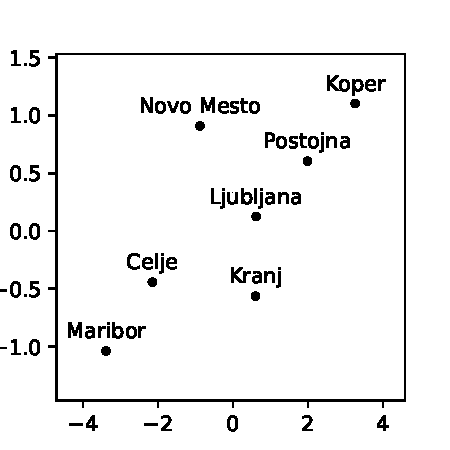
\includegraphics[width=\linewidth]{figs/060-tsne-mesta.pdf}
    \caption{Dvodimenzionalna vložitev s t-SNE.}
    \label{fig:tsne}
\end{marginfigure}

\section{Vložitve s silami}

Oglejmo si še tretji pristop. Obravnavamo ga zato, ker se po izhodišču precej razlikuje od prejšnjih dveh in ker je zelo uveljavljen na področju vizualizacije omrežij. Pristop predpostavi, da so primeri točke, med katerimi delujejo sile. Pari primerov, za katere poznamo razdalje,
%
Tu uvedemo še pomembno razliko glede na prejšnje primere: doslej smo obravnavali podatke, pri katerih so bile razdalje podane za vse pare primerov, kar pa za metode s silami ni nujno. Pogosto namreč zadošča, da poznamo razdalje ali povezave le za izbrane pare.
%
povežemo z ``vzmetmi'', ki skušajo ohranjati predpisano dolžino, hkrati pa med vsemi pari deluje še odbojna sila, ki preprečuje, da bi se točke preveč zgostile. Položaj točk v ravnini nato dobimo z iskanjem ravnovesja sil, ki ga poiščemo z minimizacijo ustrezne energijske funkcije. Čeprav je tak pristop bil razvit na področju vizualizacije omrežij, kjer želimo pregledno razporediti vozlišča grafa, ga enako uspešno uporabimo tudi za vložitve podatkov.

Kot prej, naj bo $y_i \in \mathbb{R}^2$ znova položaj primera $i$ v ravnini. Za pare primerov $(i,j)$, za katere poznamo razdaljo $d_{ij}$, uvedemo ``vzmetno'' energijo
\[
E_{\text{vzmeti}} = \frac{1}{|E|} \sum_{(i,j)\in E} \bigl( \|y_i - y_j\| - d_{ij} \bigr)^2,
\]
kjer $E$ označuje množico parov z znanimi razdaljami. Ta člen sili povezane pare, da v vložitvi ohranjajo predpisane razdalje.

Med vsemi pari primerov hkrati deluje še odbojna sila, ki jo opišemo z energijo
\[
E_{\text{odboj}} = \frac{1}{\binom{n}{2}} \sum_{i<j} \frac{1}{\|y_i - y_j\|},
\]

Skupno energijo zapišemo kot vsoto obeh členov
\[
E = E_{\text{vzmeti}} + C \, E_{\text{odboj}},
\]
kjer konstanta \(C\) določa relativni vpliv odbojnega člena. Rešitev so takšni položaji točk $y_i$, ki to skupno energijo minimizirajo.

Zgornja kriterijska funkcija je na prvi pogled še najbolj podobna tej, ki jo uporablja MDS. A podobnost je zgolj navidezna in velja le, ko so razdalje podane za vse pare. Pri MDS en sam člen enakovredno obravnava vse pare primerov in skuša globalno ohraniti vse razdalje. Pri silno vodenih vložitvah pa se kriterijska funkcija razcepi na več delov: vzmeti delujejo le med izbranimi pari (npr.\ povezanimi v omrežju) in skrbijo za lokalno strukturo, odboj pa deluje med vsemi pari in preprečuje zgoščanje točk. S tem dobimo ravnovesje med lokalnim ohranjanjem razdalj in globalnim razmikom točk, kar vodi do bistveno drugačnih vložitev kot pri MDS.

Tokrat je implementacijska koda, pač zaradi dveh členov kriterijske funkcije in potrebnih normalizacij, malce daljša:

\vspace*{3mm}
\begin{lstlisting}
class ForceDirectedLayout:
    def __init__(self, items, rep_strength=5000.0):
        random.seed(100)
        self.items = sorted(items)
        self.rep_strength = rep_strength

        self.pos = {
            i: [Value(random.uniform(-1, 1)) for _ in range(2)]
            for i in self.items
        }

    def parameters(self):
        return [p for pos in self.pos.values() for p in pos]

    def d(self, a, b):
        dx = self.pos[a][0] - self.pos[b][0]
        dy = self.pos[a][1] - self.pos[b][1]
        return (dx ** 2 + dy ** 2 + Value(1e-6)) ** 0.5

    def loss(self, edges, target_lengths):
        # springs between connected pairs
        E = edges
        L = target_lengths
        spring = Value(0.0)
        nE = len(E)

        for (a, b), t in zip(E, L):
            dist = self.d(a, b)
            spring += (dist - Value(t)) ** 2

        spring = spring / Value(nE)

        # repulsion between all pairs
        rep = Value(0.0)
        N = len(self.items)
        cnt = 0

        for i in range(N):
            for j in range(i + 1, N):
                a = self.items[i]
                b = self.items[j]
                dist = self.d(a, b)
                rep +=  dist ** (-1)
                cnt += 1

        rep = rep * self.rep_strength / cnt
        
        return spring + rep
\end{lstlisting}

Na prav enak način kot pri MDS in t-SNE pridobimo tudi vložitve s silami. Tudi tu je konvergenca hitra, dobljena vizualizacija pa presenetljivo podobna tistim, ki jih dobimo s prejšnjima metodama:
\vspace*{3mm}
\begin{lstlisting}
model = ForceDirectedLayout(items, rep_strength=5000.0)
model = train(model, pairs, targets, n_epochs=3000,
    learning_rate=0.05, report_every=100)
\end{lstlisting}

Če želimo dodatno preprečiti, da bi celotna konfiguracija ``odplavala'' stran od izhodišča, dodamo še šibek centrirni člen
\marginnote{Smo tak centrirni člen v prejšnjih poglavjih že omenjali? Na primer pri linearni regresiji? Regularizacija!}
\[
E_{\text{center}} = \frac{1}{n} \sum_{i=1}^n \|y_i\|^2,
\]
Skupno energijo zdaj zapišemo kot vsoto vseh treh členov
\[
E = E_{\text{vzmeti}} + C\,E_{\text{odboj}} + \lambda\,E_{\text{center}},
\]
kjer z nastavitvijo vrednosti konstante $\lambda$ določimo vpliv centrirnega člena. V kodi spremenimo le zadnji del metode \texttt{loss}
\vspace*{3mm}
\begin{lstlisting}
        # centering loss
        cent = Value(0.0)
        for i in self.items:
            x, y = self.pos[i]
            cent += x * x + y * y

        cent = self.cent_strength * cent / N

        return spring + rep + cent
\end{lstlisting}
in k inicializaciji razreda dodamo nastavitev \texttt{self.cent\_strength}. V naši implementaciji smo njeno vrednost nastavili na $0.001$ in pri tako določenem problemu prav velikega vpliva ni imela.

\section{Povezava t-SNE z vložitvami s silami}

Tehniko t-SNE smo predstavili kot pristop, ki minimizira Kullback-Leiblerjevo divergenco med porazdelitvama podobnosti v izvornem prostoru in prostoru vložitve:
\[
\mathcal{L}(Y) = \sum_{i \ne j} p_{ij} \log \frac{p_{ij}}{q_{ij}},
\]
kjer velja
\[
q_{ij} = \frac{(1 + \|y_i - y_j\|^2)^{-1}}{\sum_{k \ne l} (1 + \|y_k - y_l\|^2)^{-1}}.
\]
Za razumevanje dinamike optimizacije izračunamo gradient kriterijske funkcije glede na položaje točk \( y_i \). Po odvajanju (tu predstavljamo samo rezultat) dobimo
\[
\frac{\partial \mathcal{L}}{\partial y_i}
=
4 \sum_{j \ne i}
(p_{ij} - q_{ij})
\frac{(y_i - y_j)}{1 + \|y_i - y_j\|^2}.
\]
Ta izraz lahko interpretiramo kot vsoto sil, ki delujejo na točko \( y_i \). Gradient lahko razcepimo na dva člena:
\[
\frac{\partial \mathcal{L}}{\partial y_i}
=
4 \sum_{j \ne i}
p_{ij} \frac{(y_i - y_j)}{1 + \|y_i - y_j\|^2}
-
4 \sum_{j \ne i}
q_{ij} \frac{(y_i - y_j)}{1 + \|y_i - y_j\|^2}.
\]
Prvi člen lahko v interpretaciji predstavlja privlačne sile med točkama \( i \) in \( j \), katerih jakost je sorazmerna podobnosti \( p_{ij} \) v izvornem prostoru. Te sile so največje za pare, ki so si v izvornem prostoru blizu, in vlečejo ustrezne točke v vložitvi skupaj. Drugi člen predstavlja odbojne sile, ki delujejo med vsemi pari točk in preprečujejo njihovo zgoščanje. Njihova jakost izhaja iz porazdelitve \( q_{ij} \), ki je odvisna od trenutne razporeditve točk v vložitvi.

Gradient t-SNE lahko interpretiramo kot ravnovesje med privlačnimi in odbojnimi silami. V tem smislu je t-SNE soroden vložitvam s silami, le da so interakcije določene posredno prek verjetnostnega modela. Razlika je v tem, da so pri pristopu s silami te interakcije podane neposredno z vzmetnimi in odbojnimi členi, medtem ko pri t-SNE izhajajo iz verjetnostnega modela. \marginnote{Pristop t-SNE lahko zato razumemo kot verjetnostno utemeljeno vložitev s silami, kjer ravnovesje med privlačnimi in odbojnimi silami določa končno razporeditev točk v prostoru.}
Privlačne sile pri t-SNE izrecno poudarjajo lokalne sosede preko uteži \( p_{ij} \), medtem ko oblika odbojnega člena z imenovalcem \( 1 + \|y_i - y_j\|^2 \) zagotavlja dolg doseg odboja in s tem preprečuje zgoščanje točk.

\section{O implementacijah vložitvenih metod}

Implementacije v tem poglavju so namenoma poenostavljene. Njihov namen ni numerična učinkovitost, temveč jasen prikaz povezave med kriterijsko funkcijo, gradientom in končno vložitvijo. Pri tem nismo ponudili numerično najučinkovitejših rešitev. To še posebej velja za metodo t-SNE, kjer smo uporabili precej poenostavljeno različico: širino Gaussove porazdelitve smo določili z enim samim parametrom $\sigma$, enakim za vse točke, medtem ko se v praksi $\sigma_i$ prilagaja za vsak primer posebej tako, 
%
\marginnote{Parametru, ki določa število sosedov pri t-SNE-ju, v angleščini pravimo {\em perplexity}.}
da imajo vsi primeri v originalnem prostoru ``enako'' število sosedov. Poleg tega sodobne implementacije vključujejo številne izboljšave, kot so pametnejša inicializacija ter približni izračuni sil (npr. z Barnes--Hutovo aproksimacijo, kjer oddaljene točke nadomestimo z eno samo, povprečno), ki bistveno pohitrijo izvajanje pri večjih množicah podatkov. Dodaten trik je tudi zgodnje pretiravanje (angl.~\emph{early exaggeration}), kjer v začetnih iteracijah umetno povečamo vrednosti $p_{ij}$, s čimer okrepimo privlačne sile med bližnjimi točkami. Tako se skupine najprej jasno oblikujejo in ločijo, šele nato pa se njihova medsebojna razmerja natančneje uravnajo.

Podobno velja tudi za večrazsežno lestvičenje. Čeprav lahko kriterijsko funkcijo minimiziramo z gradientnim sestopom, se v praksi najpogosteje uporablja algoritem SMACOF (angl.~\emph{Scaling by MAjorizing a COmplicated Function}). Ta pristop temelji na ideji majorizacije: namesto da neposredno optimiziramo zahtevno kriterijsko funkcijo, v vsakem koraku zgradimo njeno enostavnejšo zgornjo aproksimacijo, ki jo lahko minimiziramo v zaprti obliki. Tako dobimo iterativen postopek, ki monotonno zmanjšuje vrednost kriterijske funkcije in je praviloma stabilnejši ter hitrejši od preprostega gradientnega sestopa.

Še najbliže praktični rabi je zato morda pristop z vložitvami s silami, kjer že osnovni modeli z vzmetmi in odbojem pogosto dajo uporabne rezultate. A tudi tam v praksi srečamo dodatne izboljšave, kot so uteževanje povezav, prilagajanje jakosti sil skozi čas (t.~i.\ ``ohlajanje'') in hitrejši približni izračuni odbojnih interakcij. Za praktično uporabo je pomembno predvsem to, da posamezni pristopi izhajajo iz različnih ciljev: MDS skuša ohraniti razdalje, t-SNE lokalne soseščine, metode s silami pa ravnovesje med privlačnimi in odbojnimi interakcijami.

\begin{exercise}{Vložitev novih točk.}
Razširi implementacijo vložitve tako, da pri že naučenih položajih obstoječih primerov poišče položaj nove točke zgolj iz (nekaterih) njenih razdalj oziroma podobnosti do obstoječih primerov, nato pa preveri kakovost postopka tako, da posamezne znane primere začasno odstraniš, jih ponovno vložiš kot nove in primerjaš dobljeni položaj z izvirnim.
\end{exercise}

